% ============================================================
%  J2 — APRÈS-MIDI : Sklearn, Généralisation & Overfitting
%  Julien Rolland — M2 Développement Fullstack
% ============================================================
\documentclass[aspectratio=169, 10pt]{beamer}
% ============================================================
%  PREAMBLE COMMUN — IA, Deep Learning & Machine Learning
%  Julien Rolland — M2 Développement Fullstack
% ============================================================

% --- Langue & encodage ---
\usepackage[utf8]{inputenc}
\usepackage[T1]{fontenc}
\usepackage{babel}
\babelprovide[import, main]{french}

% --- Thème Beamer ---
\usetheme{Madrid}
\usecolortheme{default}

% Palette de bleu académique
\definecolor{jedy_blue}{RGB}{0, 51, 102}       % bleu foncé principal
\definecolor{jedy_mid}{RGB}{0, 102, 179}        % bleu moyen accent
\definecolor{jedy_light}{RGB}{204, 221, 240}    % bleu très clair (fond boxes)
\definecolor{jedy_alert}{RGB}{180, 30, 30}      % rouge pour alertes
\definecolor{jedy_example}{RGB}{0, 120, 60}     % vert pour exemples

% Application des couleurs sur le thème Madrid
\setbeamercolor{palette primary}{bg=jedy_blue, fg=white}
\setbeamercolor{palette secondary}{bg=jedy_mid, fg=white}
\setbeamercolor{palette tertiary}{bg=jedy_blue, fg=white}
\setbeamercolor{palette quaternary}{bg=jedy_blue, fg=white}
\setbeamercolor{structure}{fg=jedy_blue}
\setbeamercolor{frametitle}{bg=jedy_blue, fg=white}
\setbeamercolor{title}{bg=jedy_blue, fg=white}
\setbeamercolor{block title}{bg=jedy_mid, fg=white}
\setbeamercolor{block body}{bg=jedy_light, fg=black}
\setbeamercolor{block title alerted}{bg=jedy_alert, fg=white}
\setbeamercolor{block body alerted}{bg=jedy_light, fg=black}
\setbeamercolor{block title example}{bg=jedy_example, fg=white}
\setbeamercolor{block body example}{bg=jedy_light, fg=black}

% --- Typographie ---
\usepackage{lmodern}
\setbeamerfont{title}{size=\Large, series=\bfseries}
\setbeamerfont{frametitle}{size=\normalsize, series=\bfseries}

% --- Navigation : suppression des icônes de navigation par défaut ---
\setbeamertemplate{navigation symbols}{}

% --- Numérotation des slides ---
\setbeamertemplate{footline}{%
  \leavevmode%
  \hbox{%
    \begin{beamercolorbox}[wd=.333\paperwidth,ht=2.25ex,dp=1ex,center]{author in head/foot}%
      \usebeamerfont{author in head/foot}\insertshortauthor
    \end{beamercolorbox}%
    \begin{beamercolorbox}[wd=.334\paperwidth,ht=2.25ex,dp=1ex,center]{title in head/foot}%
      \usebeamerfont{title in head/foot}\insertshorttitle
    \end{beamercolorbox}%
    \begin{beamercolorbox}[wd=.333\paperwidth,ht=2.25ex,dp=1ex,right]{date in head/foot}%
      \usebeamerfont{date in head/foot}
      \insertframenumber{} / \inserttotalframenumber\hspace*{2ex}
    \end{beamercolorbox}%
  }%
  \vskip0pt%
}

% --- Maths ---
\usepackage{amsmath, amssymb, amsthm}
\usepackage{bm}          % vecteurs en gras : \bm{w}

% --- Code source ---
\usepackage{listings}
\usepackage{xcolor}

\lstdefinestyle{pythonstyle}{
  language=Python,
  basicstyle=\ttfamily\footnotesize,
  keywordstyle=\color{jedy_blue}\bfseries,
  commentstyle=\color{gray}\itshape,
  stringstyle=\color{jedy_example},
  numberstyle=\tiny\color{gray},
  numbers=left,
  numbersep=5pt,
  frame=single,
  framerule=0.4pt,
  rulecolor=\color{jedy_light},
  backgroundcolor=\color{jedy_light!40},
  breaklines=true,
  showstringspaces=false,
  tabsize=4,
}
\lstset{style=pythonstyle}

% Alias pratique pour code inline
\newcommand{\code}[1]{\texttt{\small#1}}

% --- Graphiques ---
\usepackage{graphicx}
\usepackage{tikz}
\usetikzlibrary{arrows.meta, positioning, shapes.geometric, fit, calc}
\usepackage{pgfplots}
\pgfplotsset{compat=1.18}

% --- Tableaux ---
\usepackage{booktabs}
\usepackage{array}

% --- Icônes (optionnel, nécessite fontawesome5) ---
% \usepackage{fontawesome5}

% --- Macros ML/DL courantes ---
\newcommand{\R}{\mathbb{R}}
\newcommand{\E}{\mathbb{E}}
\newcommand{\Loss}{\mathcal{L}}
\newcommand{\dataset}{\mathcal{D}}
\newcommand{\X}{\mathbf{X}}
\newcommand{\y}{\mathbf{y}}
\newcommand{\w}{\mathbf{w}}
\newcommand{\W}{\mathbf{W}}
\newcommand{\grad}{\nabla}
\newcommand{\T}{^{\top}}         % transposée : \X\T
\newcommand{\lr}{\alpha}         % learning rate
\newcommand{\norm}[1]{\left\|#1\right\|}

% Encadré "Objectif pédagogique" en début de section
\newenvironment{objectif}{%
  \begin{alertblock}{Objectif}%
}{%
  \end{alertblock}%
}

% --- Infos du cours (remplacer dans chaque slides.tex) ---
\author[J. Rolland]{Julien Rolland}
\institute[Jedy]{Formation M2 Développement Fullstack}


\title[Généralisation \& Overfitting]{Sklearn, Généralisation \& Overfitting}
\subtitle{Jour 2 --- Après-midi}
\date{Jour 2}

% ============================================================
\begin{document}
% ============================================================

\begin{frame}
  \titlepage
\end{frame}

\begin{frame}{Plan du module}
  \tableofcontents
\end{frame}

% ============================================================
\section{Le Vrai Objectif : Généraliser}
% ============================================================

\begin{frame}{Le Vrai Objectif : Généraliser}
  \begin{columns}[T]
    \begin{column}{0.48\textwidth}
      \begin{alertblock}{Le Piège}
        \begin{itemize}
          \item Minimiser $J(\Theta, X_{\text{train}})$ = problème résolu
          \item La performance sur le train \textbf{ne compte pas}
        \end{itemize}
      \end{alertblock}

      \smallskip
      \begin{block}{Ce qu'on veut vraiment}
        \begin{itemize}
          \item Données \textbf{non-vues} (unseen data)
          \item Capter la loi sous-jacente
          \item Ignorer le bruit du dataset
        \end{itemize}
      \end{block}
    \end{column}
    \begin{column}{0.48\textwidth}
      \begin{exampleblock}{Définition}
        \textbf{Généralisation :} capacité à performer
        sur des exemples jamais vus pendant l'entraînement.
      \end{exampleblock}

      \smallskip
      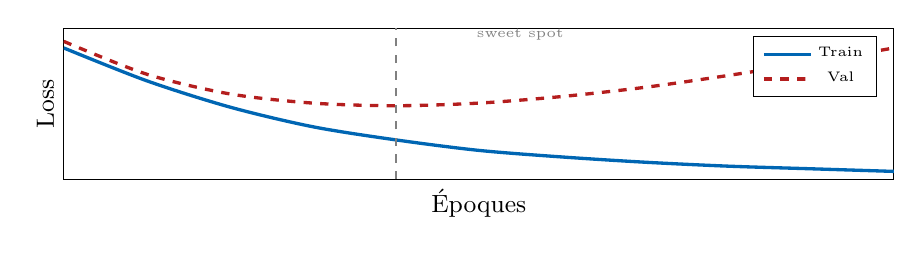
\begin{tikzpicture}
        \begin{axis}[
          width=\linewidth, height=3.5cm,
          xlabel={\small Époques},
          ylabel={\small Loss},
          xmin=0, xmax=10, ymin=0, ymax=1.15,
          xtick=\empty, ytick=\empty,
          legend style={font=\tiny, at={(0.98,0.95)}, anchor=north east},
          every axis plot/.append style={line width=1.2pt},
        ]
          \addplot[color=jedy_mid, smooth] coordinates {
            (0,1.0)(1,0.75)(2,0.55)(3,0.40)(4,0.30)
            (5,0.22)(6,0.17)(7,0.13)(8,0.10)(9,0.08)(10,0.06)
          };
          \addlegendentry{Train}
          \addplot[color=jedy_alert, dashed, smooth] coordinates {
            (0,1.05)(1,0.80)(2,0.65)(3,0.58)(4,0.56)
            (5,0.58)(6,0.63)(7,0.70)(8,0.79)(9,0.89)(10,1.00)
          };
          \addlegendentry{Val}
          \draw[gray, dashed, line width=0.6pt] (axis cs:4,0) -- (axis cs:4,1.15);
          \node[font=\tiny, gray] at (axis cs:5.5,1.10) {sweet spot};
        \end{axis}
      \end{tikzpicture}
    \end{column}
  \end{columns}
\end{frame}

% ============================================================
\section{L'Ennemi N°1 : l'Overfitting}
% ============================================================

\begin{frame}{Underfitting vs Overfitting}
  \begin{columns}[T]
    \begin{column}{0.32\textwidth}
      \begin{block}{Underfitting}
        \begin{itemize}
          \item Modèle trop \textbf{simple} --- biais élevé
          \item Train $\approx$ Val $\Rightarrow$
                \textcolor{jedy_alert}{toutes deux élevées}
        \end{itemize}
      \end{block}
      \smallskip
      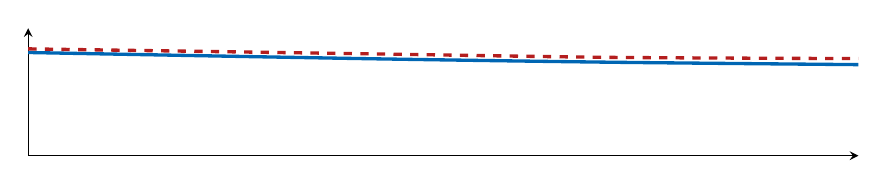
\begin{tikzpicture}
        \begin{axis}[
          width=\linewidth, height=3.2cm,
          xmin=0, xmax=10, ymin=0, ymax=1.05,
          xtick=\empty, ytick=\empty,
          axis lines=left,
          every axis plot/.append style={line width=1.2pt},
        ]
          \addplot[jedy_mid, smooth, forget plot] coordinates {
            (0,0.85)(4,0.80)(7,0.77)(10,0.75)
          };
          \addplot[jedy_alert, dashed, smooth, forget plot] coordinates {
            (0,0.88)(4,0.84)(7,0.81)(10,0.80)
          };
        \end{axis}
      \end{tikzpicture}
    \end{column}
    \begin{column}{0.32\textwidth}
      \begin{exampleblock}{Bon fit}
        \begin{itemize}
          \item Complexité adaptée aux données
          \item Train $\approx$ Val $\Rightarrow$
                \textcolor{jedy_example}{toutes deux basses}
        \end{itemize}
      \end{exampleblock}
      \smallskip
      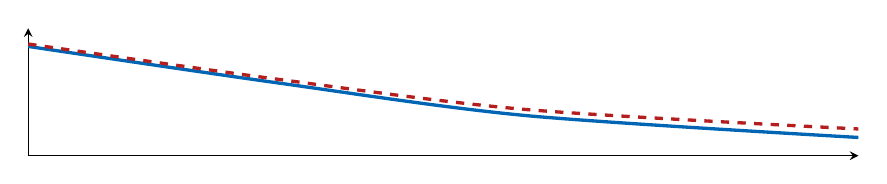
\begin{tikzpicture}
        \begin{axis}[
          width=\linewidth, height=3.2cm,
          xmin=0, xmax=10, ymin=0, ymax=1.05,
          xtick=\empty, ytick=\empty,
          axis lines=left,
          every axis plot/.append style={line width=1.2pt},
        ]
          \addplot[jedy_mid, smooth, forget plot] coordinates {
            (0,0.90)(3,0.60)(6,0.33)(10,0.15)
          };
          \addplot[jedy_alert, dashed, smooth, forget plot] coordinates {
            (0,0.92)(3,0.63)(6,0.38)(10,0.22)
          };
        \end{axis}
      \end{tikzpicture}
    \end{column}
    \begin{column}{0.32\textwidth}
      \begin{alertblock}{Overfitting}
        \begin{itemize}
          \item Modèle trop \textbf{complexe} --- variance élevée
          \item Train $\ll$ Val $\Rightarrow$
                \textcolor{jedy_alert}{Val explose}
        \end{itemize}
      \end{alertblock}
      \smallskip
      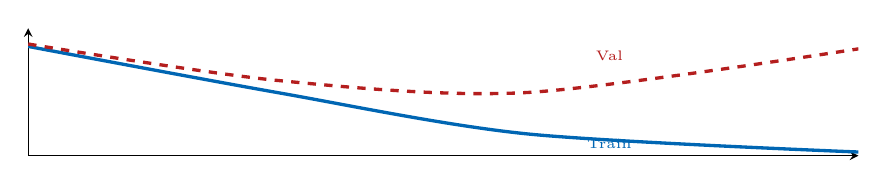
\begin{tikzpicture}
        \begin{axis}[
          width=\linewidth, height=3.2cm,
          xmin=0, xmax=10, ymin=0, ymax=1.05,
          xtick=\empty, ytick=\empty,
          axis lines=left,
          every axis plot/.append style={line width=1.2pt},
        ]
          \addplot[jedy_mid, smooth, forget plot] coordinates {
            (0,0.90)(3,0.52)(6,0.18)(10,0.03)
          };
          \addplot[jedy_alert, dashed, smooth, forget plot] coordinates {
            (0,0.92)(3,0.62)(6,0.52)(10,0.88)
          };
          \node[font=\tiny, color=jedy_mid] at (axis cs:7,0.10) {Train};
          \node[font=\tiny, color=jedy_alert] at (axis cs:7,0.82) {Val};
        \end{axis}
      \end{tikzpicture}
    \end{column}
  \end{columns}
\end{frame}

% ---

\begin{frame}{Mémorisation vs Généralisation}
  \begin{columns}[T]
    \begin{column}{0.48\textwidth}
      \begin{block}{Théorème de Cover}
        \begin{itemize}
          \item Dans $\mathbb{R}^D$, $N \leq D$ points
                sont toujours linéairement séparables
          \item Un modèle assez complexe peut
                \textbf{mémoriser} n'importe quel dataset
          \item Accuracy train $= 100\%$ ne signifie rien
        \end{itemize}
      \end{block}
    \end{column}
    \begin{column}{0.48\textwidth}
      \begin{exampleblock}{Analogie MNIST}
        \begin{itemize}
          \item Mémoriser les pixels exacts de chaque «3»
          \item Incapable de reconnaître un «3» écrit
                avec un stylo différent
          \item $\Rightarrow$ 0\% de généralisation
        \end{itemize}
      \end{exampleblock}

      \smallskip
      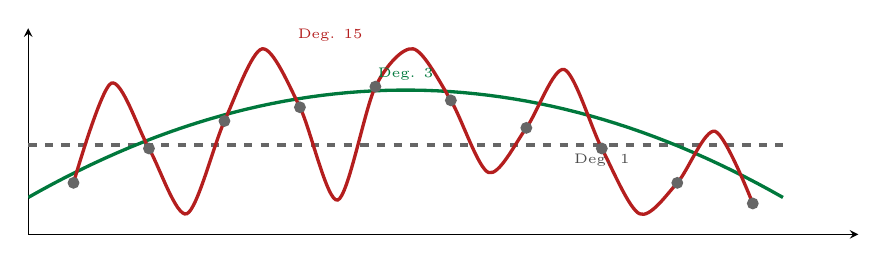
\begin{tikzpicture}
        \begin{axis}[
          width=\linewidth, height=4.2cm,
          xmin=0, xmax=5.5, ymin=-0.6, ymax=2.4,
          xtick=\empty, ytick=\empty,
          axis lines=left,
          every axis plot/.append style={line width=1.2pt},
        ]
          \addplot[only marks, mark=*, mark size=1.5pt,
                   color=black!60, forget plot] coordinates {
            (0.3,0.15)(0.8,0.65)(1.3,1.05)(1.8,1.25)(2.3,1.55)
            (2.8,1.35)(3.3,0.95)(3.8,0.65)(4.3,0.15)(4.8,-0.15)
          };
          \addplot[black!60, dashed, domain=0:5, samples=2, forget plot] {0.7};
          \addplot[jedy_example, domain=0:5, samples=60, forget plot]
            {-0.25*(x-2.5)^2+1.5};
          \addplot[jedy_alert, smooth, forget plot] coordinates {
            (0.3,0.15)(0.55,1.6)(0.8,0.65)(1.05,-0.3)
            (1.3,1.05)(1.55,2.1)(1.8,1.25)(2.05,-0.1)
            (2.3,1.55)(2.55,2.1)(2.8,1.35)(3.05,0.3)
            (3.3,0.95)(3.55,1.8)(3.8,0.65)(4.05,-0.3)
            (4.3,0.15)(4.55,0.9)(4.8,-0.15)
          };
          \node[font=\tiny, color=black!70] at (axis cs:3.8,0.48) {Deg. 1};
          \node[font=\tiny, color=jedy_example] at (axis cs:2.5,1.73) {Deg. 3};
          \node[font=\tiny, color=jedy_alert] at (axis cs:2.0,2.3) {Deg. 15};
        \end{axis}
      \end{tikzpicture}
    \end{column}
  \end{columns}
\end{frame}

% ============================================================
\section{Biais-Variance}
% ============================================================

\begin{frame}{Le Compromis Biais-Variance}
  \begin{columns}[T]
    \begin{column}{0.55\textwidth}
      \centering
      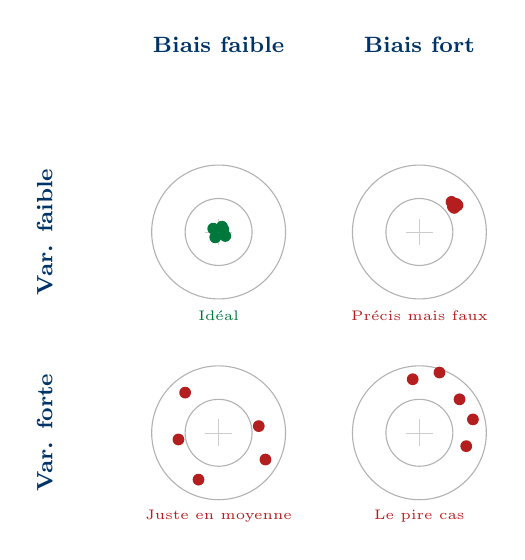
\begin{tikzpicture}[scale=0.85]
        \node[font=\footnotesize\bfseries, color=jedy_blue] at (1.5, 1.3) {Biais faible};
        \node[font=\footnotesize\bfseries, color=jedy_blue] at (4.5, 1.3) {Biais fort};
        \node[font=\footnotesize\bfseries, color=jedy_blue, rotate=90] at (-1.1,-1.5) {Var. faible};
        \node[font=\footnotesize\bfseries, color=jedy_blue, rotate=90] at (-1.1,-4.5) {Var. forte};

        % Board 1 : low bias, low var
        \draw[gray!60, thin] (1.5,-1.5) circle (1.0);
        \draw[gray!60, thin] (1.5,-1.5) circle (0.5);
        \draw[gray!40, very thin] (1.3,-1.5)--(1.7,-1.5) (1.5,-1.7)--(1.5,-1.3);
        \foreach \dx/\dy in {0.05/0.08,-0.08/0.05,0.10/-0.06,-0.05/-0.08,0.07/0.04}
          { \fill[jedy_example] ({1.5+\dx},{-1.5+\dy}) circle (2.5pt); }
        \node[font=\tiny, color=jedy_example] at (1.5,-2.75) {Idéal};

        % Board 2 : high bias, low var
        \draw[gray!60, thin] (4.5,-1.5) circle (1.0);
        \draw[gray!60, thin] (4.5,-1.5) circle (0.5);
        \draw[gray!40, very thin] (4.3,-1.5)--(4.7,-1.5) (4.5,-1.7)--(4.5,-1.3);
        \foreach \dx/\dy in {0.50/0.38,0.55/0.42,0.48/0.45,0.57/0.40,0.52/0.36}
          { \fill[jedy_alert] ({4.5+\dx},{-1.5+\dy}) circle (2.5pt); }
        \node[font=\tiny, color=jedy_alert] at (4.5,-2.75) {Précis mais faux};

        % Board 3 : low bias, high var
        \draw[gray!60, thin] (1.5,-4.5) circle (1.0);
        \draw[gray!60, thin] (1.5,-4.5) circle (0.5);
        \draw[gray!40, very thin] (1.3,-4.5)--(1.7,-4.5) (1.5,-4.7)--(1.5,-4.3);
        \foreach \dx/\dy in {0.60/0.10,-0.50/0.60,-0.30/-0.70,0.70/-0.40,-0.60/-0.10}
          { \fill[jedy_alert] ({1.5+\dx},{-4.5+\dy}) circle (2.5pt); }
        \node[font=\tiny, color=jedy_alert] at (1.5,-5.75) {Juste en moyenne};

        % Board 4 : high bias, high var
        \draw[gray!60, thin] (4.5,-4.5) circle (1.0);
        \draw[gray!60, thin] (4.5,-4.5) circle (0.5);
        \draw[gray!40, very thin] (4.3,-4.5)--(4.7,-4.5) (4.5,-4.7)--(4.5,-4.3);
        \foreach \dx/\dy in {0.60/0.50,-0.10/0.80,0.70/-0.20,0.30/0.90,0.80/0.20}
          { \fill[jedy_alert] ({4.5+\dx},{-4.5+\dy}) circle (2.5pt); }
        \node[font=\tiny, color=jedy_alert] at (4.5,-5.75) {Le pire cas};
      \end{tikzpicture}
    \end{column}
    \begin{column}{0.42\textwidth}
      \begin{block}{En Machine Learning}
        \begin{itemize}
          \item \textbf{Biais} : erreur systématique\\
                {\small modèle trop simple}
          \item \textbf{Variance} : sensibilité aux données\\
                {\small modèle trop complexe}
        \end{itemize}
        \medskip\centering
        $\text{Erreur} = \text{Biais}^2 + \text{Variance} + \varepsilon$
      \end{block}
      \smallskip
      \begin{exampleblock}{Leviers}
        \begin{itemize}
          \item \textbf{Complexité} du modèle
          \item \textbf{Régularisation} ($\lambda$)
          \item \textbf{Volume} de données
        \end{itemize}
      \end{exampleblock}
    \end{column}
  \end{columns}
\end{frame}

% ============================================================
\section{Méthodologie : Train / Validation / Test}
% ============================================================

\begin{frame}{Le Split Standard}
  \centering
  
\begin{tikzpicture}
    \node[font=\small, color=jedy_blue] at (5.0,1.2) {Dataset complet};

    \fill[jedy_mid]     (0,   0) rectangle (7.0, 0.9);
    \fill[jedy_example] (7.0, 0) rectangle (8.5, 0.9);
    \fill[jedy_alert]   (8.5, 0) rectangle (10.0,0.9);

    \node[white, font=\small\bfseries]    at (3.5,  0.45) {Train};
    \node[white, font=\tiny\bfseries]     at (7.75, 0.45) {Val};
    \node[white, font=\tiny\bfseries]     at (9.25, 0.45) {Test};

    \node[font=\footnotesize, color=jedy_mid]     at (3.5,  -0.3) {70\%};
    \node[font=\footnotesize, color=jedy_example] at (7.75, -0.3) {15\%};
    \node[font=\footnotesize, color=jedy_alert]   at (9.25, -0.3) {15\%};
  \end{tikzpicture}

  \medskip
  \begin{columns}[T]
    \begin{column}{0.52\textwidth}
      \begin{block}{3 ensembles distincts}
        \begin{enumerate}
          \item \textbf{Train} --- ajuster les paramètres $\Theta$
          \item \textbf{Validation} --- choix du modèle et des hyperparamètres
          \item \textbf{Test} --- mesure finale
        \end{enumerate}
      \end{block}
    \end{column}
    \begin{column}{0.44\textwidth}
      \begin{alertblock}{Règle d'or : Data Leakage}
        Ne \textbf{jamais} entraîner sur le test set.\\
        Ne \textbf{jamais} utiliser le test pour choisir les HP.\\
        Le test set doit rester \textbf{invisible}.
      \end{alertblock}
    \end{column}
  \end{columns}
\end{frame}

% ============================================================
\section{Cross-Validation}
% ============================================================

\begin{frame}{K-Fold Cross-Validation}
  \begin{columns}[T]
    \begin{column}{0.50\textwidth}
      \begin{alertblock}{Le Problème}
        \begin{itemize}
          \item Peu de données $\Rightarrow$ split instable
          \item Un seul val set $\Rightarrow$ variance élevée de l'estimation
        \end{itemize}
      \end{alertblock}

      \smallskip
      \begin{block}{Solution : K-Fold}
        \begin{itemize}
          \item Découper le train en $K$ morceaux (\textit{folds})
          \item $K$ rotations : chaque fold sert de validation
          \item Score final = moyenne sur $K$ runs
          \item Utilisation maximale des données disponibles
        \end{itemize}
      \end{block}
    \end{column}
    \begin{column}{0.46\textwidth}
      \centering
      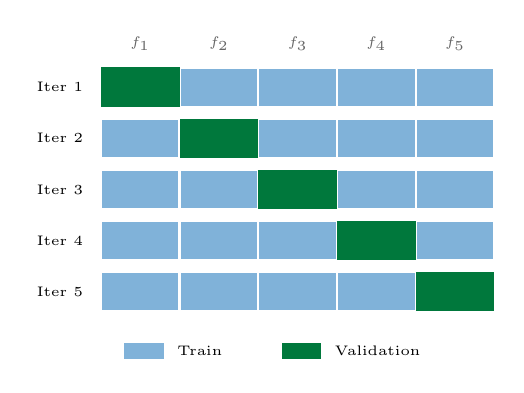
\begin{tikzpicture}
        \foreach \f/\fn in {0/1, 1/2, 2/3, 3/4, 4/5} {
          \node[font=\tiny, color=black!60] at ({(\f+0.5)}, 0.3) {$f_{\fn}$};
        }
        \foreach \k/\ki in {0/1, 1/2, 2/3, 3/4, 4/5} {
          \foreach \f in {0,...,4} {
            \fill[jedy_mid!50] ({\f},{-\k*0.65}) rectangle ({(\f+1)},{-\k*0.65-0.5});
            \draw[white, line width=0.8pt]
              ({\f},{-\k*0.65}) rectangle ({(\f+1)},{-\k*0.65-0.5});
          }
          \fill[jedy_example] ({\k},{-\k*0.65}) rectangle ({(\k+1)},{-\k*0.65-0.5});
          \node[font=\tiny, anchor=east] at (-0.1,{-\k*0.65-0.25}) {Iter \ki};
        }
        \fill[jedy_mid!50]  (0.3,-3.7) rectangle (0.8,-3.5);
        \node[font=\tiny, anchor=west] at (0.85,-3.6) {Train};
        \fill[jedy_example] (2.3,-3.7) rectangle (2.8,-3.5);
        \node[font=\tiny, anchor=west] at (2.85,-3.6) {Validation};
      \end{tikzpicture}

      \smallskip
      $\displaystyle s = \frac{1}{K}\sum_{k=1}^{K} s_k$
    \end{column}
  \end{columns}
\end{frame}

% ============================================================
\section{Scikit-Learn}
% ============================================================

\begin{frame}{Scikit-Learn}
  \begin{columns}[T]
    \begin{column}{0.50\textwidth}
      \begin{block}{La bibliothèque ML de référence}
        \begin{itemize}
          \item Open-source, basée sur NumPy / SciPy
          \item Standard de l'industrie pour le ML classique
          \item Interface cohérente pour tous les algorithmes
        \end{itemize}
      \end{block}
      \smallskip
      \begin{exampleblock}{Ce qu'elle couvre}
        \begin{itemize}
          \item \textbf{Prétraitement} : scaling, encodage, imputation
          \item \textbf{Modèles} : régression, classification, clustering
          \item \textbf{Validation} : cross-validation, grid search
          \item \textbf{Métriques} : accuracy, F1, AUC, ...
        \end{itemize}
      \end{exampleblock}
    \end{column}
    \begin{column}{0.46\textwidth}
      \centering
      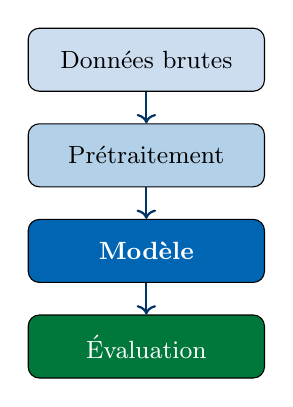
\begin{tikzpicture}[node distance=0.4cm]
        \node[draw, fill=jedy_light, rounded corners=4pt, font=\small,
              align=center, minimum width=3cm, minimum height=0.8cm]
              (raw) {Données brutes};
        \node[draw, fill=jedy_mid!30, rounded corners=4pt, font=\small,
              align=center, minimum width=3cm, minimum height=0.8cm,
              below=0.4cm of raw]
              (pre) {Prétraitement};
        \node[draw, fill=jedy_mid, text=white, rounded corners=4pt,
              font=\small\bfseries, align=center,
              minimum width=3cm, minimum height=0.8cm,
              below=0.4cm of pre]
              (mod) {Modèle};
        \node[draw, fill=jedy_example, text=white, rounded corners=4pt,
              font=\small, align=center,
              minimum width=3cm, minimum height=0.8cm,
              below=0.4cm of mod]
              (eva) {Évaluation};
        \draw[->, thick, jedy_blue] (raw) -- (pre);
        \draw[->, thick, jedy_blue] (pre) -- (mod);
        \draw[->, thick, jedy_blue] (mod) -- (eva);
      \end{tikzpicture}
    \end{column}
  \end{columns}
\end{frame}

% ---

\begin{frame}[fragile]{L'API Estimator}
  \begin{block}{Interface universelle}
    \begin{tabular}{@{}ll@{}}
      \texttt{.fit(X, y)}         & Apprend les paramètres internes sur les données d'entraînement \\[3pt]
      \texttt{.predict(X)}        & Prédit les labels / valeurs pour de nouveaux exemples \\[3pt]
      \texttt{.transform(X)}      & Applique la transformation apprise (scalers, encodeurs\ldots) \\[3pt]
      \texttt{.fit\_transform(X)} & \texttt{.fit()} + \texttt{.transform()} en une seule passe \\[3pt]
      \texttt{.score(X, y)}       & Retourne une métrique : accuracy (classif), $R^2$ (régression) \\
    \end{tabular}
  \end{block}
  \smallskip
  \begin{lstlisting}[style=pythonstyle]
from sklearn.linear_model import LogisticRegression
from sklearn.preprocessing import StandardScaler

scaler = StandardScaler()
X_tr = scaler.fit_transform(X_train)  # fit sur train uniquement
X_te = scaler.transform(X_test)       # applique la meme normalisation

clf = LogisticRegression()
clf.fit(X_tr, y_train)
print(clf.score(X_te, y_test))
  \end{lstlisting}
\end{frame}

% ---

\begin{frame}[fragile]{Pipeline}
  \begin{columns}[T]
    \begin{column}{0.96\textwidth}
      \begin{block}{Principe}
        \begin{itemize}
          \item Enchaîner Scaler $\to$ Modèle
          \item \texttt{.fit()} appliqué séquentiellement
          \item Compatible avec la cross-validation
        \end{itemize}
      \end{block}
    \end{column}
  \end{columns}

  \medskip
  \begin{lstlisting}[style=pythonstyle]
from sklearn.pipeline import Pipeline
from sklearn.preprocessing import StandardScaler
from sklearn.linear_model import LogisticRegression

pipe = Pipeline([
    ('scaler', StandardScaler()),
    ('clf',    LogisticRegression()),
])

pipe.fit(X_train, y_train)
print(pipe.score(X_test, y_test))
  \end{lstlisting}
\end{frame}

% ---

\begin{frame}[fragile]{train\_test\_split \& cross\_val\_score}
  \begin{columns}[T]
    \begin{column}{0.48\textwidth}
      \begin{block}{\texttt{train\_test\_split}}
        \begin{itemize}
          \item Découpe aléatoire du dataset
          \item \texttt{test\_size} : proportion du test set
          \item \texttt{random\_state} : reproductibilité
          \item \texttt{stratify} : préserve les proportions de classes
        \end{itemize}
      \end{block}
    \end{column}
    \begin{column}{0.48\textwidth}
      \begin{exampleblock}{\texttt{cross\_val\_score}}
        \begin{itemize}
          \item K-Fold intégré, compatible Pipeline
          \item Retourne un score par fold
          \item \texttt{cv} : nombre de folds
          \item \texttt{scoring} : métrique (\texttt{'accuracy'}, ...)
        \end{itemize}
      \end{exampleblock}
    \end{column}
  \end{columns}

  \medskip
  \begin{lstlisting}[style=pythonstyle]
from sklearn.model_selection import train_test_split, cross_val_score

X_train, X_test, y_train, y_test = train_test_split(
    X, y, test_size=0.2, random_state=42, stratify=y)

scores = cross_val_score(pipe, X_train, y_train, cv=5)
print(f"CV: {scores.mean():.3f} +/- {scores.std():.3f}")
  \end{lstlisting}
\end{frame}


% ---

\begin{frame}{Modèles supervisés}
  \begin{columns}[T]
    \begin{column}{0.48\textwidth}
      \begin{block}{Classification}
        \begin{itemize}
          \item \texttt{LogisticRegression} --- linéaire, rapide
          \item \texttt{SVC} --- à noyau, puissant
          \item \texttt{KNeighborsClassifier} --- basé distance
          \item \texttt{RandomForestClassifier} --- ensemble
          \item \texttt{GradientBoostingClassifier} --- boosting
        \end{itemize}
      \end{block}
    \end{column}
    \begin{column}{0.48\textwidth}
      \begin{exampleblock}{Régression}
        \begin{itemize}
          \item \texttt{LinearRegression} --- OLS
          \item \texttt{Ridge} / \texttt{Lasso} --- régularisés
          \item \texttt{SVR} --- à noyau
          \item \texttt{RandomForestRegressor}
          \item \texttt{GradientBoostingRegressor}
        \end{itemize}
      \end{exampleblock}
    \end{column}
  \end{columns}
  \medskip
  \begin{alertblock}{Interface universelle}
    \centering
    \texttt{.fit(X, y)} \qquad \texttt{.predict(X)} \qquad \texttt{.score(X, y)}
  \end{alertblock}
\end{frame}

% ---

\begin{frame}[fragile]{Prétraitement : \texttt{sklearn.preprocessing}}
  \begin{columns}[T]
    \begin{column}{0.48\textwidth}
      \begin{block}{Normalisation}
        \begin{itemize}
          \item \texttt{StandardScaler} --- $\mu=0,\;\sigma=1$
          \item \texttt{MinMaxScaler} --- $[0,\,1]$
          \item \texttt{RobustScaler} --- robuste aux outliers
        \end{itemize}
      \end{block}
      \smallskip
      \begin{exampleblock}{Encodage \& Imputation}
        \begin{itemize}
          \item \texttt{OneHotEncoder} --- catégorielles $\to$ binaires
          \item \texttt{LabelEncoder} --- labels $\to$ entiers
          \item \texttt{SimpleImputer} --- valeurs manquantes
        \end{itemize}
      \end{exampleblock}
    \end{column}
    \begin{column}{0.48\textwidth}
      \begin{lstlisting}[style=pythonstyle]
from sklearn.preprocessing import (
    StandardScaler, OneHotEncoder,
    SimpleImputer,
)

# normalisation
scaler = StandardScaler()
X_sc = scaler.fit_transform(X_train)

# valeurs manquantes
imp = SimpleImputer(strategy='mean')
X_cl = imp.fit_transform(X_train)

# variables categorielles
enc = OneHotEncoder()
X_cat = enc.fit_transform(X_train)
      \end{lstlisting}
    \end{column}
  \end{columns}
\end{frame}

% ---

\begin{frame}[fragile]{Métriques : \texttt{sklearn.metrics}}
  \begin{columns}[T]
    \begin{column}{0.48\textwidth}
      \begin{block}{Classification}
        \begin{itemize}
          \item \texttt{accuracy\_score}
          \item \texttt{f1\_score} --- macro / weighted
          \item \texttt{confusion\_matrix}
          \item \texttt{classification\_report}
          \item \texttt{roc\_auc\_score}
        \end{itemize}
      \end{block}
      \smallskip
      \begin{exampleblock}{Régression}
        \begin{itemize}
          \item \texttt{mean\_squared\_error} (MSE)
          \item \texttt{mean\_absolute\_error} (MAE)
          \item \texttt{r2\_score} --- coefficient $R^2$
        \end{itemize}
      \end{exampleblock}
    \end{column}
    \begin{column}{0.48\textwidth}
      \begin{lstlisting}[style=pythonstyle]
from sklearn.metrics import (
    accuracy_score,
    classification_report,
    confusion_matrix,
)

y_pred = clf.predict(X_test)

print(accuracy_score(y_test, y_pred))
print(classification_report(
    y_test, y_pred))
print(confusion_matrix(
    y_test, y_pred))
      \end{lstlisting}
    \end{column}
  \end{columns}
\end{frame}

% ---

\begin{frame}[fragile]{Recherche d'hyperparamètres}
  \begin{columns}[T]
    \begin{column}{0.48\textwidth}
      \begin{block}{\texttt{GridSearchCV}}
        \begin{itemize}
          \item Teste toutes les combinaisons
          \item Cross-validation intégrée
          \item Compatible Pipeline
        \end{itemize}
      \end{block}
      \smallskip
      \begin{exampleblock}{\texttt{RandomizedSearchCV}}
        \begin{itemize}
          \item Échantillonnage aléatoire de l'espace
          \item Plus rapide sur de grands espaces
          \item \texttt{n\_iter} itérations
        \end{itemize}
      \end{exampleblock}
    \end{column}
    \begin{column}{0.48\textwidth}
      \begin{lstlisting}[style=pythonstyle]
from sklearn.model_selection import (
    GridSearchCV)
from sklearn.svm import SVC

param_grid = {
    'C':      [0.1, 1, 10],
    'kernel': ['linear', 'rbf'],
}

grid = GridSearchCV(
    SVC(), param_grid, cv=5,
    scoring='accuracy')
grid.fit(X_train, y_train)

print(grid.best_params_)
print(grid.best_score_)
      \end{lstlisting}
    \end{column}
  \end{columns}
\end{frame}

% ============================================================
\section*{Récapitulatif}
% ============================================================

\begin{frame}{Récapitulatif}
  \begin{columns}[T]
    \begin{column}{0.48\textwidth}
      \begin{block}{Généralisation}
        \small\begin{itemize}
          \item Objectif : données \textbf{non vues}, pas le train
          \item Underfitting --- biais élevé, modèle trop simple
          \item Overfitting --- variance élevée, modèle trop complexe
          \item Compromis biais-variance : le \textit{sweet spot}
        \end{itemize}
      \end{block}
      \smallskip
      \begin{exampleblock}{Méthodologie}
        \small\begin{itemize}
          \item Split \textbf{Train / Val / Test} --- test intouchable
          \item \textbf{K-Fold} --- estimation robuste, peu de données
        \end{itemize}
      \end{exampleblock}
    \end{column}
    \begin{column}{0.48\textwidth}
      \begin{alertblock}{API Scikit-Learn}
        \small\begin{itemize}
          \item \texttt{.fit()} / \texttt{.predict()} / \texttt{.score()}
          \item \texttt{Pipeline} --- prétraitement + modèle chaînés
          \item \texttt{GridSearchCV} --- recherche d'hyperparamètres
        \end{itemize}
      \end{alertblock}
      \smallskip
      \begin{block}{Modules clés}
        \small\begin{itemize}
          \item \texttt{preprocessing} --- scalers, encodeurs
          \item \texttt{linear\_model} / \texttt{ensemble} / \texttt{svm}
          \item \texttt{metrics} --- accuracy, F1, $R^2$
          \item \texttt{model\_selection} --- CV, GridSearch
        \end{itemize}
      \end{block}
    \end{column}
  \end{columns}
\end{frame}

% ============================================================
\end{document}
